
\documentclass[aspectratio=169,10pt]{beamer}

\usepackage[utf8]{inputenc}
\usepackage[T1]{fontenc}
\usepackage{lmodern}
\usepackage{amsmath,amssymb}
\usepackage{booktabs,tabularx,array,adjustbox}
\usepackage{tikz,pgfplots}
\usepackage[most]{tcolorbox}
\usepackage{graphicx,xcolor,ragged2e}
\usepackage{listings}
\pgfplotsset{compat=1.18}
\usetikzlibrary{arrows.meta,positioning,calc,decorations.pathreplacing,angles,quotes}

% ---------- Palette (template Pertemuan 2/5) ----------
\definecolor{DeepNavy}{HTML}{073B4C}
\definecolor{Teal}{HTML}{118AB2}
\definecolor{SoftBlue}{HTML}{E8F4FA}
\definecolor{Orange}{HTML}{F26B21}
\definecolor{SoftOrange}{HTML}{FFF0E6}
\definecolor{Mint}{HTML}{D9F2EC}
\definecolor{Purple}{HTML}{6A4C93}
\definecolor{SoftPurple}{HTML}{F2ECFA}
\definecolor{Gold}{HTML}{F7B801}
\definecolor{SoftGold}{HTML}{FFF7D6}
\definecolor{GrayText}{HTML}{4A5568}
\definecolor{LightLine}{HTML}{D9E2EC}
\definecolor{RedAccent}{HTML}{D1495B}

% ---------- Beamer ----------
\setbeamertemplate{navigation symbols}{}
\setbeamercolor{normal text}{fg=DeepNavy,bg=white}
\setbeamercolor{frametitle}{fg=DeepNavy,bg=white}
\setbeamerfont{frametitle}{size=\Large,series=\bfseries}
\setbeamertemplate{frametitle}{%
  \vspace{0.25em}\insertframetitle\par
  \vspace{-0.25em}\tikz{\draw[Orange,line width=1.15pt] (0,0)--(1.15,0);}\vspace{-0.48em}
}
\setbeamertemplate{footline}{%
\leavevmode\hbox{%
\begin{beamercolorbox}[wd=.46\paperwidth,ht=2.2ex,dp=1ex,leftskip=1em]{}\scriptsize MA25-31017 Pemodelan Komputasi dan Analisis Numerik\end{beamercolorbox}%
\begin{beamercolorbox}[wd=.36\paperwidth,ht=2.2ex,dp=1ex,center]{}\scriptsize Program Studi Matematika ITERA\end{beamercolorbox}%
\begin{beamercolorbox}[wd=.18\paperwidth,ht=2.2ex,dp=1ex,rightskip=1em plus1fil]{}\scriptsize \insertframenumber/\inserttotalframenumber\end{beamercolorbox}}%
}

% ---------- Boxes ----------
\tcbset{enhanced,boxrule=.7pt,arc=2mm,left=2mm,right=2mm,top=1mm,bottom=1mm,fonttitle=\bfseries,before skip=1pt,after skip=1pt}
\newtcolorbox{bluebox}[1][]{colback=SoftBlue,colframe=Teal,title=#1}
\newtcolorbox{orangebox}[1][]{colback=SoftOrange,colframe=Orange,title=#1}
\newtcolorbox{greenbox}[1][]{colback=Mint,colframe=DeepNavy!55!Teal,title=#1}
\newtcolorbox{purplebox}[1][]{colback=SoftPurple,colframe=Purple,title=#1}
\newtcolorbox{goldbox}[1][]{colback=SoftGold,colframe=Gold!80!black,title=#1}
\newcommand{\highlight}[1]{\textcolor{Orange}{\textbf{#1}}}
\newcommand{\smallgray}[1]{\textcolor{GrayText}{\scriptsize #1}}

% ---------- Code ----------
\lstdefinestyle{matlabstyle}{
  language=Matlab,
  basicstyle=\ttfamily\scriptsize,
  keywordstyle=\color{Teal}\bfseries,
  commentstyle=\color{GrayText},
  stringstyle=\color{Purple},
  showstringspaces=false,
  columns=fullflexible,
  keepspaces=true,
  frame=single,
  rulecolor=\color{LightLine},
  backgroundcolor=\color{SoftBlue!35},
  xleftmargin=1mm,
  xrightmargin=1mm,
  aboveskip=1mm,
  belowskip=1mm
}

\begin{document}

% ============ 1. COVER ============
\begin{frame}[plain]
\begin{tikzpicture}[remember picture,overlay]
  \fill[SoftBlue] (current page.north west) rectangle ([xshift=.48\paperwidth]current page.south west);
  \fill[white] ([xshift=.48\paperwidth]current page.north west) rectangle (current page.south east);
\end{tikzpicture}
\vspace{0.52cm}
\begin{columns}[T,totalwidth=\textwidth]
\begin{column}{.44\textwidth}
{\fontsize{21}{24}\selectfont\bfseries Persamaan Diferensial\\Biasa (PDB)}\par
\vspace{0.10cm}
\tikz{\draw[Orange,line width=1.5pt] (0,0)--(1.9,0);}\par
\vspace{0.14cm}
{\large Masalah Nilai Awal:\\Metode Euler, Heun, dan Runge--Kutta}\par
\vspace{0.38cm}
\small MA25-31017 \textbullet\ Pertemuan 9\par
\small Program Studi Matematika\par
\small Institut Teknologi Sumatera\par
\vspace{0.27cm}
\textbf{Dosen Pengampu}\par
Rifky Fauzi\par
Dear Michiko Mutiara Noor
\end{column}
\begin{column}{.52\textwidth}
\vspace{0.02cm}
\begin{tikzpicture}
\begin{axis}[width=\linewidth,height=.55\textheight,axis lines=middle,
  xmin=-.1,xmax=2.15,ymin=.5,ymax=4.9,
  xlabel={$x$},ylabel={$y$},xtick={0,.5,1,1.5,2},ytick=\empty,
  grid=both,grid style={LightLine!55},
  tick label style={font=\scriptsize},label style={font=\scriptsize}]
\addplot[domain=0:2,Teal,very thick,samples=120]{-0.5*x^4+4*x^3-10*x^2+8.5*x+1};
\addplot[Orange,very thick,mark=*,mark size=1.6pt]
 coordinates {(0,1) (.5,5.25) (1,5.875) (1.5,5.125) (2,4.5)};
\addplot[Purple,very thick,dashed,mark=square*,mark size=1.4pt]
 coordinates {(0,1) (.5,3.4375) (1,3.375) (1.5,2.6875) (2,2.5)};
\node[font=\scriptsize,Teal,anchor=south west] at (axis cs:1.38,2.18) {solusi eksak};
\node[font=\scriptsize,Orange,anchor=south west] at (axis cs:1.45,4.4) {Euler};
\node[font=\scriptsize,Purple,anchor=north west] at (axis cs:1.45,2.95) {Heun};
\end{axis}
\end{tikzpicture}
\par\vspace{-0.12cm}
\centering\smallgray{Satu masalah nilai awal, beberapa cara membaca kemiringan.}
\end{column}
\end{columns}
\end{frame}

% ============ 2 ============
\begin{frame}{Mengapa PDB dihampiri secara numerik?}
\scriptsize
\begin{columns}[T,totalwidth=\textwidth]
\begin{column}{.50\textwidth}
\begin{bluebox}[PDB sebagai laju perubahan]
Banyak fenomena dimodelkan dalam bentuk
\[
\boxed{y'=f(x,y),\qquad y(x_0)=y_0}
\]
misalnya pertumbuhan populasi, peluruhan, atau dinamika sistem mekanik.
\end{bluebox}
\begin{orangebox}[Ide numerik]
Mulai dari titik awal $(x_0,y_0)$, gunakan informasi \highlight{kemiringan} $f(x,y)$ untuk melangkah sedikit demi sedikit ke depan.
\end{orangebox}
\begin{greenbox}[Yang menentukan kualitas solusi]
\begin{itemize}
\item cara menaksir kemiringan,
\item ukuran langkah $h$,
\item akumulasi galat sepanjang langkah.
\end{itemize}
\end{greenbox}
\end{column}
\begin{column}{.46\textwidth}
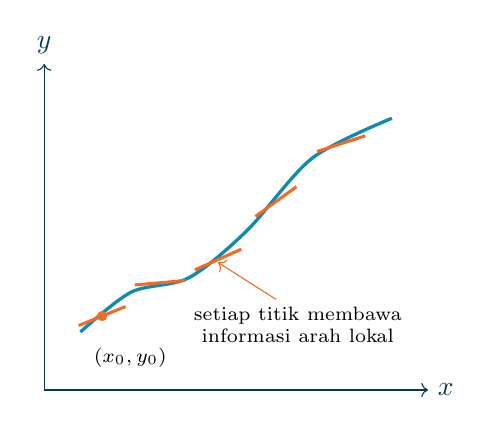
\begin{tikzpicture}[scale=.92]
\draw[->,DeepNavy] (0,0)--(5.3,0) node[right]{$x$};
\draw[->,DeepNavy] (0,0)--(0,4.5) node[above]{$y$};
\draw[Teal,very thick] plot[smooth] coordinates {(0.5,.8) (1.2,1.35) (2,1.55) (2.8,2.2) (3.7,3.2) (4.8,3.75)};
\foreach \x/\y/\ang in {.8/1.02/22,1.6/1.48/5,2.4/1.8/24,3.2/2.6/36,4.1/3.4/18}{
  \draw[Orange,line width=1.1pt,rotate around={\ang:(\x,\y)}] (\x-.35,\y)--(\x+.35,\y);
}
\fill[Orange] (.8,1.02) circle (2pt);
\node[align=center,font=\scriptsize] at (3.5,.9) {setiap titik membawa\\informasi arah lokal};
\draw[->,Orange] (3.2,1.25)--(2.4,1.76);
\node[font=\scriptsize,anchor=north west] at (.55,.72) {$(x_0,y_0)$};
\end{tikzpicture}
\vspace{1mm}
\begin{purplebox}[Pertanyaan]
Jika kemiringan berubah cepat, apakah satu kemiringan di awal interval masih cukup?
\end{purplebox}
\end{column}
\end{columns}
\end{frame}

% ============ 3 ============
\begin{frame}{Deret Taylor sebagai mesin pembentuk rumus}
\scriptsize
\begin{columns}[T,totalwidth=\textwidth]
\begin{column}{.54\textwidth}
\begin{bluebox}[Ekspansi maju]
Untuk $x_{i+1}=x_i+h$,
\[
\begin{aligned}
y(x_{i+1})=&\,y(x_i)+y'(x_i)h\\
&+\frac{y''(x_i)}{2!}h^2
+\frac{y^{(3)}(x_i)}{3!}h^3+\cdots
\end{aligned}
\]
\end{bluebox}
\begin{orangebox}[Potong setelah turunan pertama]
\[
y(x_{i+1})\approx y(x_i)+y'(x_i)h
\]
Suku yang dibuang membentuk \highlight{galat pemotongan}.
\end{orangebox}
\end{column}
\begin{column}{.42\textwidth}
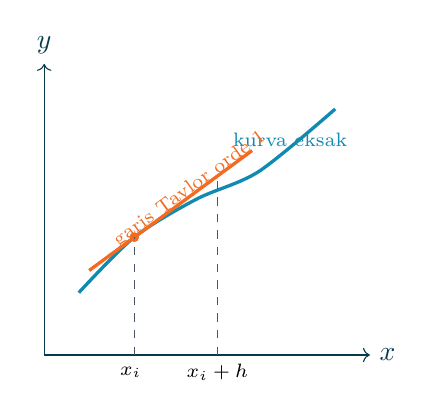
\begin{tikzpicture}[scale=.88]
\draw[->,DeepNavy] (0,0)--(4.7,0) node[right]{$x$};
\draw[->,DeepNavy] (0,0)--(0,4.2) node[above]{$y$};
\draw[Teal,very thick] plot[smooth] coordinates {(0.5,.9) (1.3,1.7) (2.2,2.25) (3.1,2.65) (4.2,3.55)};
\fill[Orange] (1.3,1.7) circle (2pt);
\draw[Orange,very thick] (.65,1.22)--(3.0,2.95);
\draw[dashed,GrayText] (1.3,0)--(1.3,1.7);
\draw[dashed,GrayText] (2.5,0)--(2.5,2.58);
\node[font=\scriptsize] at (1.25,-.25) {$x_i$};
\node[font=\scriptsize] at (2.5,-.25) {$x_i+h$};
\node[font=\scriptsize,Teal] at (3.55,3.1) {kurva eksak};
\node[font=\scriptsize,Orange,rotate=36] at (2.1,2.4) {garis Taylor orde 1};
\end{tikzpicture}
\begin{goldbox}[Intuisi]
Euler adalah Taylor orde satu yang diterapkan berulang kali.
\end{goldbox}
\end{column}
\end{columns}
\end{frame}

% ============ 4 ============
\begin{frame}{Metode Euler}
\scriptsize
\begin{columns}[T,totalwidth=\textwidth]
\begin{column}{.48\textwidth}
\begin{bluebox}[Formula iterasi]
Karena $y'(x_i)=f(x_i,y_i)$,
\[
\boxed{y_{i+1}=y_i+h\,f(x_i,y_i)}
\]
\end{bluebox}
\begin{greenbox}[Makna setiap komponen]
\begin{tabularx}{\linewidth}{lX}
$y_i$ & nilai saat ini\\
$f(x_i,y_i)$ & kemiringan di titik saat ini\\
$h$ & ukuran langkah\\
$y_{i+1}$ & prediksi pada langkah berikutnya
\end{tabularx}
\end{greenbox}
\end{column}
\begin{column}{.48\textwidth}
\begin{orangebox}[Struktur galat]
Pemotongan Taylor setelah suku linear memberi
\[
\text{galat lokal}=O(h^2),
\qquad
\text{galat global}=O(h).
\]
\end{orangebox}
\begin{purplebox}[Konsekuensi]
Memperkecil $h$ biasanya memperbaiki akurasi, tetapi jumlah langkah dan biaya komputasi meningkat.
\end{purplebox}
\end{column}
\end{columns}
\vspace{1mm}
\begin{center}
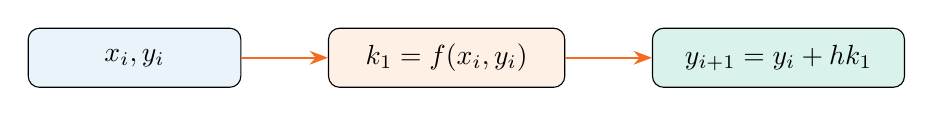
\begin{tikzpicture}[>=Stealth]
\node[draw,rounded corners,fill=SoftBlue,minimum width=2.7cm,minimum height=.75cm] (a) {$x_i,y_i$};
\node[draw,rounded corners,fill=SoftOrange,right=1.1cm of a,minimum width=3.0cm,minimum height=.75cm] (b) {$k_1=f(x_i,y_i)$};
\node[draw,rounded corners,fill=Mint,right=1.1cm of b,minimum width=3.2cm,minimum height=.75cm] (c) {$y_{i+1}=y_i+h k_1$};
\draw[->,thick,Orange] (a)--(b);
\draw[->,thick,Orange] (b)--(c);
\end{tikzpicture}
\end{center}
\end{frame}

% ============ 5 ============
\begin{frame}{Visualisasi satu langkah Euler}
\scriptsize
\begin{columns}[T,totalwidth=\textwidth]
\begin{column}{.60\textwidth}
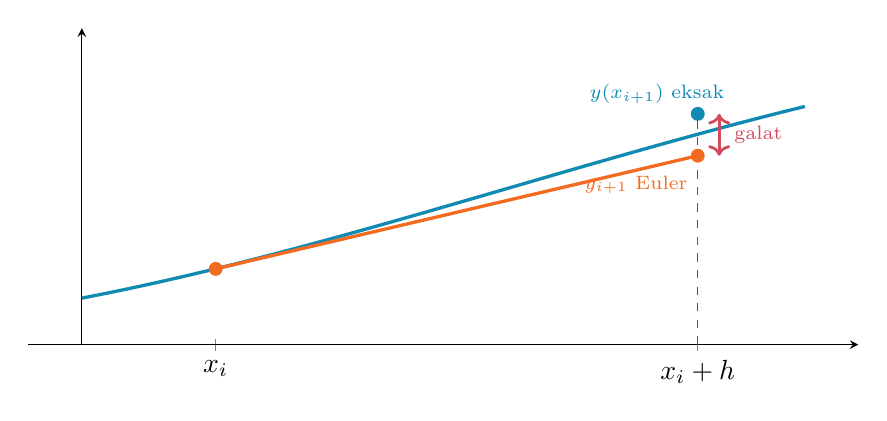
\begin{tikzpicture}
\begin{axis}[width=\linewidth,height=5.6cm,axis lines=middle,
xmin=-.1,xmax=1.45,ymin=.2,ymax=1.9,
xtick={.25,1.15},xticklabels={$x_i$,$x_i+h$},
ytick=\empty,grid=none,label style={font=\scriptsize}]
\addplot[domain=0:1.35,Teal,very thick,samples=120]{.45+.55*x+.36*x^2-.15*x^3};
\addplot[Orange,very thick] coordinates {(.25,.607) (1.15,1.215)};
\addplot[only marks,mark=*,mark size=2.3pt,Orange] coordinates {(.25,.607) (1.15,1.215)};
\addplot[only marks,mark=*,mark size=2.3pt,Teal] coordinates {(1.15,1.44)};
\draw[dashed,GrayText] (axis cs:1.15,.2)--(axis cs:1.15,1.44);
\draw[<->,RedAccent,line width=1pt] (axis cs:1.19,1.215)--(axis cs:1.19,1.44);
\node[font=\scriptsize,RedAccent,anchor=west] at (axis cs:1.2,1.33) {galat};
\node[font=\scriptsize,Orange,anchor=north west] at (axis cs:.92,1.16) {$y_{i+1}$ Euler};
\node[font=\scriptsize,Teal,anchor=south west] at (axis cs:.93,1.44) {$y(x_{i+1})$ eksak};
\end{axis}
\end{tikzpicture}
\end{column}
\begin{column}{.36\textwidth}
\begin{goldbox}[Pertanyaan kelas]
Euler mempertahankan kemiringan awal sepanjang satu interval.

\vspace{1mm}
Apa yang terjadi pada akumulasi galat jika $h$ diperbesar?
\end{goldbox}
\begin{orangebox}[Kunci observasi]
Kesalahan bukan hanya karena satu langkah, tetapi juga karena nilai hasil langkah sebelumnya dipakai kembali pada langkah berikutnya.
\end{orangebox}
\end{column}
\end{columns}
\end{frame}

% ============ 6 ============
\begin{frame}{Ukuran langkah $h$: lebih kecil, biasanya lebih dekat}
\scriptsize
\begin{columns}[T,totalwidth=\textwidth]
\begin{column}{.66\textwidth}
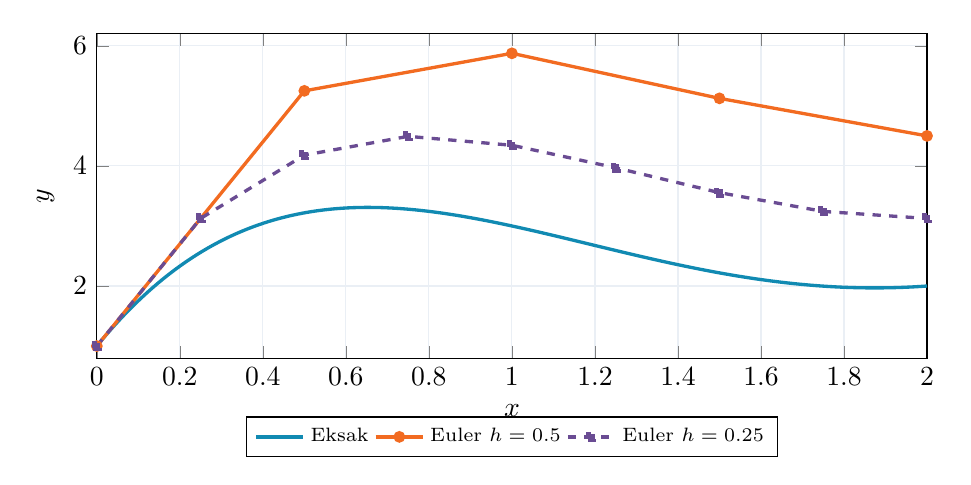
\begin{tikzpicture}
\begin{axis}[width=\linewidth,height=5.7cm,
xlabel={$x$},ylabel={$y$},xmin=0,xmax=2,ymin=.8,ymax=6.2,
grid=both,grid style={LightLine!55},
legend style={font=\scriptsize,at={(.5,-.18)},anchor=north,legend columns=3}]
\addplot[domain=0:2,Teal,very thick,samples=150]{-0.5*x^4+4*x^3-10*x^2+8.5*x+1};
\addlegendentry{Eksak}
\addplot[Orange,very thick,mark=*,mark size=1.5pt]
 coordinates {(0,1) (.5,5.25) (1,5.875) (1.5,5.125) (2,4.5)};
\addlegendentry{Euler $h=0.5$}
\addplot[Purple,very thick,dashed,mark=square*,mark size=1.2pt]
 coordinates {(0,1) (.25,3.125) (.5,4.1796875) (.75,4.4921875) (1,4.34375) (1.25,3.96875) (1.5,3.5546875) (1.75,3.2421875) (2,3.125)};
\addlegendentry{Euler $h=0.25$}
\end{axis}
\end{tikzpicture}
\end{column}
\begin{column}{.30\textwidth}
\begin{bluebox}[Yang berubah]
Saat $h$ diperkecil:
\begin{itemize}
\item garis Euler ``di-reset'' lebih sering,
\item kemiringan diperbarui lebih sering,
\item galat global cenderung turun.
\end{itemize}
\end{bluebox}
\begin{purplebox}[Trade-off]
Akurasi naik, tetapi jumlah evaluasi fungsi juga naik.
\end{purplebox}
\end{column}
\end{columns}
\end{frame}

% ============ 7 ============
\begin{frame}{Contoh hitung Euler}
\scriptsize
\begin{bluebox}[Masalah nilai awal]
\[
y'=-2x^3+12x^2-20x+8.5,\qquad y(0)=1,
\]
hitung dari $x=0$ ke $x=0.5$ dengan $h=0.5$. Diketahui $y(0.5)=3.21875$.
\end{bluebox}
\begin{columns}[T,totalwidth=\textwidth]
\begin{column}{.48\textwidth}
\begin{orangebox}[Langkah Euler]
\[
x_0=0,\qquad y_0=1
\]
\[
f(0,1)=8.5
\]
\[
\boxed{y_1=1+(8.5)(0.5)=5.25}
\]
\end{orangebox}
\end{column}
\begin{column}{.48\textwidth}
\begin{purplebox}[Evaluasi]
\[
|e|=|5.25-3.21875|=2.03125
\]
\[
e_r\approx 63.1\%
\]
Kemiringan awal $8.5$ terlalu besar jika dipakai untuk merepresentasikan seluruh interval $[0,0.5]$.
\end{purplebox}
\end{column}
\end{columns}
\end{frame}

% ============ 8 ============
\begin{frame}{Menaikkan akurasi: Metode Heun}
\scriptsize
\begin{columns}[T,totalwidth=\textwidth]
\begin{column}{.48\textwidth}
\begin{bluebox}[Ide prediktor-korektor]
Jangan hanya memakai kemiringan awal.
\begin{enumerate}
\item Prediksi titik akhir dengan Euler.
\item Hitung kemiringan di titik prediksi.
\item Rata-ratakan dua kemiringan.
\end{enumerate}
\end{bluebox}
\begin{orangebox}[Formula]
Prediktor:
\[
y_{i+1}^{(0)}=y_i+h\,f(x_i,y_i)
\]
Korektor:
\[
\boxed{
y_{i+1}
=y_i+\frac{h}{2}\left[
f(x_i,y_i)+f(x_{i+1},y_{i+1}^{(0)})
\right]}
\]
\end{orangebox}
\end{column}
\begin{column}{.48\textwidth}
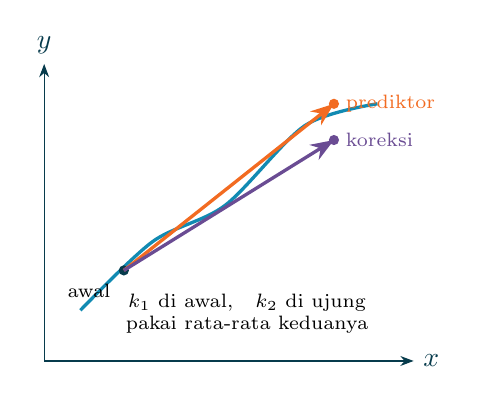
\begin{tikzpicture}[>=Stealth,scale=.92]
\draw[->,DeepNavy] (0,0)--(5.1,0) node[right]{$x$};
\draw[->,DeepNavy] (0,0)--(0,4.1) node[above]{$y$};
\draw[Teal,very thick] plot[smooth] coordinates {(.5,.7) (1.5,1.65) (2.5,2.15) (3.6,3.25) (4.6,3.55)};
\fill[DeepNavy] (1.1,1.25) circle (2pt);
\draw[Orange,very thick,->] (1.1,1.25)--(4.0,3.55);
\fill[Orange] (4.0,3.55) circle (2pt);
\draw[Purple,very thick,->] (1.1,1.25)--(4.0,3.05);
\fill[Purple] (4.0,3.05) circle (2pt);
\node[font=\scriptsize,anchor=north east] at (1.05,1.2) {awal};
\node[font=\scriptsize,Orange,anchor=west] at (4.03,3.55) {prediktor};
\node[font=\scriptsize,Purple,anchor=west] at (4.03,3.05) {koreksi};
\node[font=\scriptsize,align=center] at (2.8,.65) {$k_1$ di awal,\quad $k_2$ di ujung\\pakai rata-rata keduanya};
\end{tikzpicture}
\begin{greenbox}[Akurasi]
Heun memiliki galat global $O(h^2)$.
\end{greenbox}
\end{column}
\end{columns}
\end{frame}

% ============ 9 ============
\begin{frame}{Contoh yang sama: Euler vs Heun}
\scriptsize
\begin{columns}[T,totalwidth=\textwidth]
\begin{column}{.48\textwidth}
\begin{bluebox}[Prediktor]
\[
k_1=f(0,1)=8.5
\]
\[
y_1^{(0)}=1+(8.5)(0.5)=5.25
\]
Di ujung interval,
\[
k_2=f(0.5,5.25)=1.25.
\]
\end{bluebox}
\begin{orangebox}[Korektor]
\[
y_1
=1+\frac{0.5}{2}(8.5+1.25)
=\boxed{3.4375}.
\]
\end{orangebox}
\end{column}
\begin{column}{.48\textwidth}
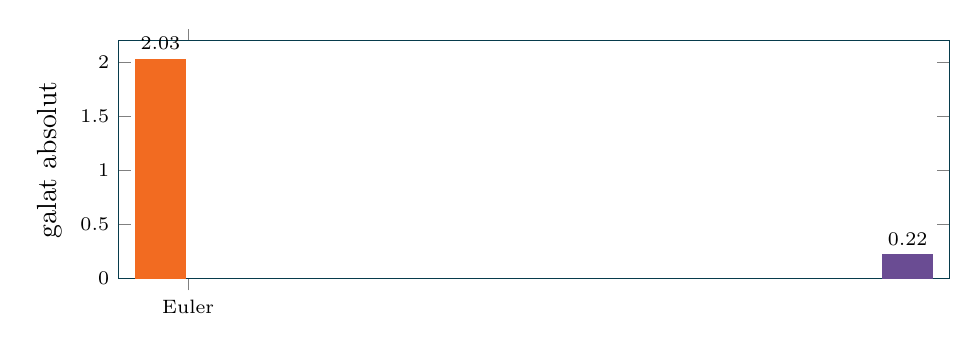
\begin{tikzpicture}
\begin{axis}[ybar,width=\linewidth,height=4.6cm,
symbolic x coords={Euler,Heun},
xtick=data,ymin=0,ymax=2.2,
ylabel={galat absolut},
nodes near coords,
nodes near coords style={font=\scriptsize},
bar width=18pt,axis line style={DeepNavy},tick label style={font=\scriptsize}]
\addplot[fill=Orange,draw=Orange] coordinates {(Euler,2.03125)};
\addplot[fill=Purple,draw=Purple] coordinates {(Heun,0.21875)};
\end{axis}
\end{tikzpicture}
\vspace{-1mm}
\begin{greenbox}[Hasil]
Nilai eksak $=3.21875$.

Heun jauh lebih dekat karena memakai informasi kemiringan di dua lokasi dalam interval.
\end{greenbox}
\end{column}
\end{columns}
\end{frame}

% ============ 10 ============
\begin{frame}{Metode Runge--Kutta Orde 2}
\scriptsize
\begin{bluebox}[Bentuk umum RK2]
\[
y_{i+1}=y_i+h(a_1k_1+a_2k_2),
\]
\[
k_1=f(x_i,y_i),\qquad
k_2=f(x_i+p_1h,\ y_i+q_{11}k_1h).
\]
\end{bluebox}
\begin{columns}[T,totalwidth=\textwidth]
\begin{column}{.56\textwidth}
\begin{tabularx}{\linewidth}{lcccc}
\toprule
Varian & $a_1$ & $a_2$ & $p_1$ & $q_{11}$\\
\midrule
Heun & $1/2$ & $1/2$ & $1$ & $1$\\
Titik tengah & $0$ & $1$ & $1/2$ & $1/2$\\
Ralston & $1/3$ & $2/3$ & $3/4$ & $3/4$\\
\bottomrule
\end{tabularx}
\end{column}
\begin{column}{.40\textwidth}
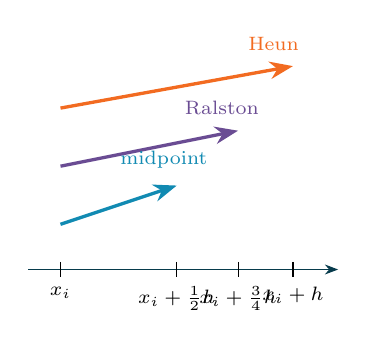
\begin{tikzpicture}[>=Stealth,scale=.82]
\draw[->,DeepNavy] (0,0)--(4.8,0);
\foreach \x/\lab in {.5/$x_i$,2.3/$x_i+\frac12h$,3.25/$x_i+\frac34h$,4.1/$x_i+h$}{
\draw (\x,.12)--(\x,-.12) node[below,font=\scriptsize]{\lab};
}
\draw[Teal,very thick,->] (.5,.7)--(2.3,1.3);
\draw[Purple,very thick,->] (.5,1.6)--(3.25,2.15);
\draw[Orange,very thick,->] (.5,2.5)--(4.1,3.15);
\node[font=\scriptsize,Teal] at (2.1,1.7) {midpoint};
\node[font=\scriptsize,Purple] at (3.0,2.5) {Ralston};
\node[font=\scriptsize,Orange] at (3.8,3.5) {Heun};
\end{tikzpicture}
\end{column}
\end{columns}
\vspace{1mm}
\begin{goldbox}[Pesan penting]
Heun bukan metode yang berdiri sendiri dari keluarga RK: ia adalah salah satu pilihan bagaimana mengambil dan membobot kemiringan kedua.
\end{goldbox}
\end{frame}

% ============ 11 ============
\begin{frame}{Runge--Kutta Orde 4: empat kemiringan dalam satu langkah}
\scriptsize
\begin{columns}[T,totalwidth=\textwidth]
\begin{column}{.48\textwidth}
\begin{bluebox}[Empat evaluasi]
\[
\begin{aligned}
k_1&=f(x_i,y_i),\\
k_2&=f\left(x_i+\tfrac12h,\ y_i+\tfrac12hk_1\right),\\
k_3&=f\left(x_i+\tfrac12h,\ y_i+\tfrac12hk_2\right),\\
k_4&=f(x_i+h,\ y_i+hk_3).
\end{aligned}
\]
\[
\boxed{
y_{i+1}=y_i+\frac{h}{6}(k_1+2k_2+2k_3+k_4)}
\]
\end{bluebox}
\end{column}
\begin{column}{.48\textwidth}
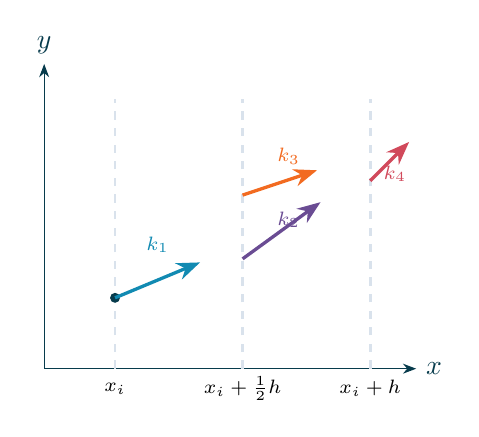
\begin{tikzpicture}[>=Stealth,scale=.9]
\draw[->,DeepNavy] (0,0)--(5.25,0) node[right]{$x$};
\draw[->,DeepNavy] (0,0)--(0,4.3) node[above]{$y$};
\draw[dashed,LightLine,line width=1pt] (1,0)--(1,3.8);
\draw[dashed,LightLine,line width=1pt] (2.8,0)--(2.8,3.8);
\draw[dashed,LightLine,line width=1pt] (4.6,0)--(4.6,3.8);
\node[font=\scriptsize] at (1,-.28) {$x_i$};
\node[font=\scriptsize] at (2.8,-.28) {$x_i+\frac12h$};
\node[font=\scriptsize] at (4.6,-.28) {$x_i+h$};
\fill[DeepNavy] (1,1.0) circle (2pt);
\draw[Teal,very thick,->] (1,1.0)--(2.2,1.5);
\draw[Purple,very thick,->] (2.8,1.55)--(3.9,2.35);
\draw[Orange,very thick,->] (2.8,2.45)--(3.85,2.8);
\draw[RedAccent,very thick,->] (4.6,2.65)--(5.15,3.2);
\node[font=\scriptsize,Teal] at (1.6,1.75) {$k_1$};
\node[font=\scriptsize,Purple] at (3.45,2.1) {$k_2$};
\node[font=\scriptsize,Orange] at (3.45,3.0) {$k_3$};
\node[font=\scriptsize,RedAccent] at (4.95,2.75) {$k_4$};
\end{tikzpicture}
\begin{greenbox}[Trade-off]
RK4 memerlukan 4 evaluasi $f$ per langkah, tetapi galat globalnya $O(h^4)$.
\end{greenbox}
\end{column}
\end{columns}
\end{frame}

% ============ 12 ============
\begin{frame}[fragile]{Demo komputasi singkat}
\scriptsize
\begin{columns}[T,totalwidth=\textwidth]
\begin{column}{.55\textwidth}
\begin{lstlisting}[style=matlabstyle]
f = @(x,y) -2*x.^3 + 12*x.^2 ...
           -20*x + 8.5;
h = 0.5; x0 = 0; y0 = 1; x1 = 0.5;

% Euler
y_euler = y0 + f(x0,y0)*h;

% Heun
y_pred = y0 + f(x0,y0)*h;
slope  = (f(x0,y0)+f(x1,y_pred))/2;
y_heun = y0 + slope*h;
\end{lstlisting}
\end{column}
\begin{column}{.41\textwidth}
\begin{bluebox}[Output satu langkah]
\begin{center}
\begin{tabular}{lrr}
\toprule
Metode & $y(0.5)$ & $|e|$\\
\midrule
Eksak & 3.21875 & 0\\
Euler & 5.25000 & 2.03125\\
Heun & 3.43750 & 0.21875\\
\bottomrule
\end{tabular}
\end{center}
\end{bluebox}
\begin{purplebox}[Interpretasi]
Heun memperbaiki tebakan karena tidak menganggap kemiringan awal berlaku konstan sepanjang interval.
\end{purplebox}
\end{column}
\end{columns}
\end{frame}

% ============ 13 ============
\begin{frame}{Latihan mandiri}
\scriptsize
\begin{goldbox}[Soal 1 - Euler]
Selesaikan
\[
y'=4e^{0.8x}-0.5y,\qquad y(0)=2
\]
dari $x=0$ hingga $x=1$ dengan $h=0.5$ menggunakan Metode Euler.

Tampilkan $x_i$, $y_i$, dan nilai kemiringan pada setiap langkah.
\end{goldbox}
\vspace{1mm}
\begin{orangebox}[Soal 2 - Heun]
Gunakan masalah nilai awal yang sama. Hitung $y(1)$ dengan Metode Heun
(satu koreksi pada setiap langkah), lalu bandingkan hasil akhirnya dengan Euler.
\end{orangebox}
\vspace{1mm}
\begin{bluebox}[Catatan]
Gunakan minimal 4 angka di belakang koma selama perhitungan untuk menghindari pembulatan terlalu dini.
\end{bluebox}
\end{frame}

% ============ 14 ============
\begin{frame}{Bahan presentasi berikutnya}
\scriptsize
\begin{columns}[T,totalwidth=\textwidth]
\begin{column}{.48\textwidth}
\begin{bluebox}[Bagian A - Soal yang dibuat sendiri]
Pilih satu PDB nonlinear sederhana dan satu syarat awal.
\begin{enumerate}
\item Terapkan Euler dan Heun secara manual.
\item Gunakan minimal 2 langkah komputasi.
\item Sajikan tabel perbandingan hasil dan galat.
\end{enumerate}
\end{bluebox}
\end{column}
\begin{column}{.48\textwidth}
\begin{purplebox}[Bagian B - Kajian RK4]
Pilih satu referensi yang mengaplikasikan RK4.
\begin{enumerate}
\item Tuliskan $k_1,k_2,k_3,k_4$.
\item Jelaskan mengapa RK4 sering dipilih dibanding Euler/Heun.
\item Tampilkan grafik perbandingan hasil simulasi jika memungkinkan.
\end{enumerate}
\end{purplebox}
\end{column}
\end{columns}
\vspace{1mm}
\begin{goldbox}[Fokus presentasi]
Bukan hanya menampilkan rumus. Tunjukkan bagaimana pemilihan kemiringan dan ukuran langkah memengaruhi hasil komputasi.
\end{goldbox}
\end{frame}

\end{document}
